% Options for packages loaded elsewhere
\PassOptionsToPackage{unicode}{hyperref}
\PassOptionsToPackage{hyphens}{url}
%
\documentclass[
  9pt,
]{article}
\usepackage{amsmath,amssymb}
\usepackage{lmodern}
\usepackage{iftex}
\ifPDFTeX
  \usepackage[T1]{fontenc}
  \usepackage[utf8]{inputenc}
  \usepackage{textcomp} % provide euro and other symbols
\else % if luatex or xetex
  \usepackage{unicode-math}
  \defaultfontfeatures{Scale=MatchLowercase}
  \defaultfontfeatures[\rmfamily]{Ligatures=TeX,Scale=1}
\fi
% Use upquote if available, for straight quotes in verbatim environments
\IfFileExists{upquote.sty}{\usepackage{upquote}}{}
\IfFileExists{microtype.sty}{% use microtype if available
  \usepackage[]{microtype}
  \UseMicrotypeSet[protrusion]{basicmath} % disable protrusion for tt fonts
}{}
\makeatletter
\@ifundefined{KOMAClassName}{% if non-KOMA class
  \IfFileExists{parskip.sty}{%
    \usepackage{parskip}
  }{% else
    \setlength{\parindent}{0pt}
    \setlength{\parskip}{6pt plus 2pt minus 1pt}}
}{% if KOMA class
  \KOMAoptions{parskip=half}}
\makeatother
\usepackage{xcolor}
\usepackage[margin=1in]{geometry}
\usepackage{color}
\usepackage{fancyvrb}
\newcommand{\VerbBar}{|}
\newcommand{\VERB}{\Verb[commandchars=\\\{\}]}
\DefineVerbatimEnvironment{Highlighting}{Verbatim}{commandchars=\\\{\}}
% Add ',fontsize=\small' for more characters per line
\usepackage{framed}
\definecolor{shadecolor}{RGB}{248,248,248}
\newenvironment{Shaded}{\begin{snugshade}}{\end{snugshade}}
\newcommand{\AlertTok}[1]{\textcolor[rgb]{0.94,0.16,0.16}{#1}}
\newcommand{\AnnotationTok}[1]{\textcolor[rgb]{0.56,0.35,0.01}{\textbf{\textit{#1}}}}
\newcommand{\AttributeTok}[1]{\textcolor[rgb]{0.77,0.63,0.00}{#1}}
\newcommand{\BaseNTok}[1]{\textcolor[rgb]{0.00,0.00,0.81}{#1}}
\newcommand{\BuiltInTok}[1]{#1}
\newcommand{\CharTok}[1]{\textcolor[rgb]{0.31,0.60,0.02}{#1}}
\newcommand{\CommentTok}[1]{\textcolor[rgb]{0.56,0.35,0.01}{\textit{#1}}}
\newcommand{\CommentVarTok}[1]{\textcolor[rgb]{0.56,0.35,0.01}{\textbf{\textit{#1}}}}
\newcommand{\ConstantTok}[1]{\textcolor[rgb]{0.00,0.00,0.00}{#1}}
\newcommand{\ControlFlowTok}[1]{\textcolor[rgb]{0.13,0.29,0.53}{\textbf{#1}}}
\newcommand{\DataTypeTok}[1]{\textcolor[rgb]{0.13,0.29,0.53}{#1}}
\newcommand{\DecValTok}[1]{\textcolor[rgb]{0.00,0.00,0.81}{#1}}
\newcommand{\DocumentationTok}[1]{\textcolor[rgb]{0.56,0.35,0.01}{\textbf{\textit{#1}}}}
\newcommand{\ErrorTok}[1]{\textcolor[rgb]{0.64,0.00,0.00}{\textbf{#1}}}
\newcommand{\ExtensionTok}[1]{#1}
\newcommand{\FloatTok}[1]{\textcolor[rgb]{0.00,0.00,0.81}{#1}}
\newcommand{\FunctionTok}[1]{\textcolor[rgb]{0.00,0.00,0.00}{#1}}
\newcommand{\ImportTok}[1]{#1}
\newcommand{\InformationTok}[1]{\textcolor[rgb]{0.56,0.35,0.01}{\textbf{\textit{#1}}}}
\newcommand{\KeywordTok}[1]{\textcolor[rgb]{0.13,0.29,0.53}{\textbf{#1}}}
\newcommand{\NormalTok}[1]{#1}
\newcommand{\OperatorTok}[1]{\textcolor[rgb]{0.81,0.36,0.00}{\textbf{#1}}}
\newcommand{\OtherTok}[1]{\textcolor[rgb]{0.56,0.35,0.01}{#1}}
\newcommand{\PreprocessorTok}[1]{\textcolor[rgb]{0.56,0.35,0.01}{\textit{#1}}}
\newcommand{\RegionMarkerTok}[1]{#1}
\newcommand{\SpecialCharTok}[1]{\textcolor[rgb]{0.00,0.00,0.00}{#1}}
\newcommand{\SpecialStringTok}[1]{\textcolor[rgb]{0.31,0.60,0.02}{#1}}
\newcommand{\StringTok}[1]{\textcolor[rgb]{0.31,0.60,0.02}{#1}}
\newcommand{\VariableTok}[1]{\textcolor[rgb]{0.00,0.00,0.00}{#1}}
\newcommand{\VerbatimStringTok}[1]{\textcolor[rgb]{0.31,0.60,0.02}{#1}}
\newcommand{\WarningTok}[1]{\textcolor[rgb]{0.56,0.35,0.01}{\textbf{\textit{#1}}}}
\usepackage{graphicx}
\makeatletter
\def\maxwidth{\ifdim\Gin@nat@width>\linewidth\linewidth\else\Gin@nat@width\fi}
\def\maxheight{\ifdim\Gin@nat@height>\textheight\textheight\else\Gin@nat@height\fi}
\makeatother
% Scale images if necessary, so that they will not overflow the page
% margins by default, and it is still possible to overwrite the defaults
% using explicit options in \includegraphics[width, height, ...]{}
\setkeys{Gin}{width=\maxwidth,height=\maxheight,keepaspectratio}
% Set default figure placement to htbp
\makeatletter
\def\fps@figure{htbp}
\makeatother
\setlength{\emergencystretch}{3em} % prevent overfull lines
\providecommand{\tightlist}{%
  \setlength{\itemsep}{0pt}\setlength{\parskip}{0pt}}
\setcounter{secnumdepth}{-\maxdimen} % remove section numbering
\ifLuaTeX
\usepackage[bidi=basic]{babel}
\else
\usepackage[bidi=default]{babel}
\fi
\babelprovide[main,import]{ngerman}
% get rid of language-specific shorthands (see #6817):
\let\LanguageShortHands\languageshorthands
\def\languageshorthands#1{}
\ifLuaTeX
  \usepackage{selnolig}  % disable illegal ligatures
\fi
\IfFileExists{bookmark.sty}{\usepackage{bookmark}}{\usepackage{hyperref}}
\IfFileExists{xurl.sty}{\usepackage{xurl}}{} % add URL line breaks if available
\urlstyle{same} % disable monospaced font for URLs
\hypersetup{
  pdftitle={Widerstandsmessungen},
  pdfauthor={Milena Mensching, Justus Weyers},
  pdflang={de},
  hidelinks,
  pdfcreator={LaTeX via pandoc}}

\title{Widerstandsmessungen}
\author{Milena Mensching, Justus Weyers}
\date{2023-01-11}

\begin{document}
\maketitle

\hypertarget{experiment}{%
\section{Experiment}\label{experiment}}

\hypertarget{thema}{%
\subsection{Thema}\label{thema}}

Bestimmung von Widerständen auf direkte und indirekte Weise. Dazu werden
die Beträge der zwei zu untersuchenden Widerstände durch ablesen der
Farbcodes, durch Widerstandsmessungen mit einem Multimeter und in einem
Schaltkreis ermittelt.

\hypertarget{material}{%
\subsection{Material}\label{material}}

\begin{itemize}
\item{Zwei Multimeter}
\item{Breadboard}
\item{Jumperwire, Bananenstecker und Krokodilklemmen}
\item{Netzgerät}
\item{Zwei Widerstände unbekannter Größe}
\end{itemize}

\hypertarget{auslesen-der-widerstandsfarbcodes}{%
\subsection{Auslesen der
Widerstandsfarbcodes}\label{auslesen-der-widerstandsfarbcodes}}

Als erste Methode zur Bestimmung des Widerstandes werden die
Bauteilspezifikationen auf dem Widertstand selbst abgelesen. Im
folgenden wird von ``Widerstand 1'' und ``Widerstand 2'' gesprochen.

\begin{figure}
\centering
\includegraphics[width=\textwidth,height=0.2\textheight]{Bilder/1MOhm.png}
\caption{Foto von Widerstand 1}
\end{figure}

Die Farbreihenfolge auf dem Widerstand ist
\(Braun, Schwarz, Schwarz, Gelb, Braun\). Dementsprechend kodiert der im
Folgenden als \(R_1\) bezeichnete Widerstand für
\(R_1 = (100 \cdot 10^4\pm 1\% ) \Omega \Leftrightarrow R_1=(1,00\pm 0,01) M\Omega\).

\begin{figure}
\centering
\includegraphics[width=\textwidth,height=0.2\textheight]{Bilder/1Ohm.png}
\caption{Foto von Widerstand 2}
\end{figure}

Widerstand 2 ist als Widerstand von \(1\Omega\) gekennzeichnet. Aus
Datenblättern im Internet geht hervor, dass auch dieser eine Toleranz
von \(\pm 1 \%\) aufweist
(\url{https://de.rs-online.com/web/p/durchsteckwiderstande/1249328}).
Dies bedeutet einen Widerstand von \(R_2=(1,00 \pm 0,01)\Omega\) für
dieses Bauteil.

\hypertarget{direkte-messung}{%
\subsection{Direkte Messung}\label{direkte-messung}}

Messungen der Widerstände mit dem Multimeter liefert Werte von:

\begin{itemize}
\item $R_1 = 1,005 M\Omega$\\
\item $R_2 = 1,0 \Omega$
\end{itemize}

\hypertarget{messunsicherheiten-der-direkten-messung}{%
\subsubsection{Messunsicherheiten der direkten
Messung}\label{messunsicherheiten-der-direkten-messung}}

Die Messunsicherheit der direkten Messung ergibt sich aus der
Messunsicherheit der digitalen Skala:

\begin{equation*}
\begin{split}
u_{Skala} &=\frac{a}{2\sqrt{3}} \\
1.Widerstand: u_1 &= \frac{0,001M\Omega}{2\sqrt{3}} \approx \pm 0,00029 M\Omega \\
2.Widerstand: u_2 &= \frac{0,1\Omega}{2\sqrt{3}} \approx \pm 0,029\Omega 
\end{split}
\end{equation*}

\begin{Shaded}
\begin{Highlighting}[]
\FloatTok{0.001}\SpecialCharTok{/}\NormalTok{(}\DecValTok{2}\SpecialCharTok{*}\FunctionTok{sqrt}\NormalTok{(}\DecValTok{3}\NormalTok{)) }\CommentTok{\#Unsicherheit 1}
\end{Highlighting}
\end{Shaded}

\begin{verbatim}
## [1] 0.0002886751
\end{verbatim}

\begin{Shaded}
\begin{Highlighting}[]
\FloatTok{0.1}\SpecialCharTok{/}\NormalTok{(}\DecValTok{2}\SpecialCharTok{*}\FunctionTok{sqrt}\NormalTok{(}\DecValTok{3}\NormalTok{)) }\CommentTok{\#Unsicherheit 2}
\end{Highlighting}
\end{Shaded}

\begin{verbatim}
## [1] 0.02886751
\end{verbatim}

\hypertarget{indirekte-widerstandsmessung}{%
\subsection{Indirekte
Widerstandsmessung}\label{indirekte-widerstandsmessung}}

Die indirekte Bestimmung der Widerstände in einem Stromkreis erfolgt in
zwei Varianten. Diese Unterscheiden sich in der Art des
Schaltungsaufbaus. In Abbildung \ldots{} ist der Unterschied zwischen
den Varianten a) und b) erkennlich.

\begin{figure}
\centering
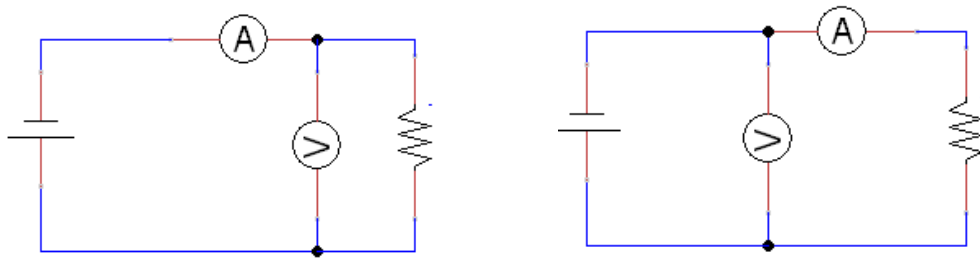
\includegraphics[width=\textwidth,height=0.1\textheight]{Bilder/Schaltkreis.png}
\caption{Schaltkreise zur indirekten Widerstandsmessung. Links: Variante
a). Rechts: Variante b). Quelle: Universität Potsdam, Institut für
Physik und Astronomie, Grundpraktikum, Skript zum Versuch E1.}
\end{figure}

In Variante a) wird das Voltmeter parallel zum Widerstand geschaltet, in
Variante b) parallel zur Spannungsquelle.

Bei der Berechnung der Widerstände aus den gemessenen Werten werden zwei
Annahmen/Vereinfachungen getroffen:

\begin{itemize}
  \item Durch das Voltmeter findet Stromfluss statt. Der tatsächliche Innenwiderstand beträgt ca. $10M\Omega$, wie Datenblättern des Messgerätes aus dem Internet entnommen und auch experimentell überprüft wurde.
  \item Das Amperemeter hat keinen Innenwiderstand. In den Datenblättern gab es keine Agaben zum Innenwiderstand des Amperemeters und auch experimentell konnte kein Widerstand bestimmt werden.
\end{itemize}

Verwendetes Datenblatt:
\url{https://asset.conrad.com/media10/add/160267/c1/-/en/000124501DS01/datasheet-124501-voltcraft-vc250-handheld-multimeter-digital-cat-iii-600-v-display-counts-2000.pdf}.

\hypertarget{aufbau-a}{%
\subsection{Aufbau (a)}\label{aufbau-a}}

Mithilfe der Kabel und des Breadboards wurde folgender Stromkreis
aufgebaut:

\begin{figure}
\centering
\includegraphics[width=\textwidth,height=0.2\textheight]{Bilder/SchaltungA.png}
\caption{Aufbau auf Breadboard für Variante a) der indirekten
Widerstandsmessung. Im Bild ist zudem bereits der Widerstand 1
eingebaut.}
\end{figure}

Folgende Werte wurden gemessen:

\begin{itemize}
\item {Widerstand 1 (Messung bei 5,0V)}
\begin{itemize}
\item {Spannung: 5,04V}
\item {5,4 $\mu$A}
\end{itemize}
\item {Widerstand 2 (Messung bei 0,6V)}
\begin{itemize}
\item {Spannung: 0,15 V}
\item {150,3 mA}
\end{itemize}
\end{itemize}

\hypertarget{geruxe4tespezifische-messunsicherheiten}{%
\subsubsection{Gerätespezifische
Messunsicherheiten}\label{geruxe4tespezifische-messunsicherheiten}}

Die Messunsicherheitem von Spannung und Strom ergeben sich aus der
Messunsicherheit der digitalen Skala

\begin{equation*}
\begin{split}
u_{Skala} &=\frac{a}{2\sqrt{3}} \\
\underline{1.Widerstand:} \\
Spannung: u_{U1a} &= \frac{0,01V}{2\sqrt{3}} \approx 0,0029 V \\
Strom: u_{I1a} &= \frac{0,1\mu A}{2\sqrt{3}} \approx 0,029\mu A \\
\underline{2.Widerstand:} \\
Spannung: u_{U2a} &= \frac{0,01V}{2\sqrt{3}} \approx 0,0029 V \\
Strom: u_{I2a} &= \frac{0,1mA}{2\sqrt{3}} \approx 0,029 mA \\
\end{split}
\end{equation*}

\begin{Shaded}
\begin{Highlighting}[]
\FloatTok{0.01}\SpecialCharTok{/}\NormalTok{(}\DecValTok{2}\SpecialCharTok{*}\FunctionTok{sqrt}\NormalTok{(}\DecValTok{3}\NormalTok{)) }\CommentTok{\#Unsicherheit Spannung 1,2}
\end{Highlighting}
\end{Shaded}

\begin{verbatim}
## [1] 0.002886751
\end{verbatim}

\begin{Shaded}
\begin{Highlighting}[]
\FloatTok{0.1}\SpecialCharTok{/}\NormalTok{(}\DecValTok{2}\SpecialCharTok{*}\FunctionTok{sqrt}\NormalTok{(}\DecValTok{3}\NormalTok{)) }\CommentTok{\#Unsicherheit Strom 1,2}
\end{Highlighting}
\end{Shaded}

\begin{verbatim}
## [1] 0.02886751
\end{verbatim}

Folglich liegen die gemessenen Größen bei:

\begin{itemize}
\item $U1a = (5,0400 \pm 0,0029)V$
\item $I1a = (5,400 \pm 0,029) \mu A$
\item $U2a = (0,1500 \pm 0,0029)V$
\item $I2a = (150,300 \pm 0,029) mA$
\end{itemize}

\hypertarget{berechnung-der-widerstuxe4nde}{%
\subsubsection{Berechnung der
Widerstände}\label{berechnung-der-widerstuxe4nde}}

Es gilt das Ohmsche Gesetz:

\(U=I\cdot R \Leftrightarrow R = \frac{U}{I}\)

\noindent \(R\) =Widerstand\\
\noindent \(U\) = Spannung\\
\noindent \(I\) = Strom

Für die Widerstände ergeben sich somit für Aufbau (a) Bestwerte von:
\begin{equation*}
\begin{split}
1. Widerstand: R=\frac{U}{I} = \frac {5,0400V}{5,4 \mu A} \approx 933333,3 \Omega \\
2.Widerstand: R=\frac{U}{I} = \frac {0,1500V}{150,3 mA} \approx 0,998004 \Omega \\
\end{split}
\end{equation*}

\begin{Shaded}
\begin{Highlighting}[]
\NormalTok{(}\FloatTok{5.04}\SpecialCharTok{/}\NormalTok{(}\FloatTok{5.4}\SpecialCharTok{*}\DecValTok{10}\SpecialCharTok{**{-}}\DecValTok{6}\NormalTok{)) }\CommentTok{\#Widerstand 1}
\end{Highlighting}
\end{Shaded}

\begin{verbatim}
## [1] 933333.3
\end{verbatim}

\begin{Shaded}
\begin{Highlighting}[]
\NormalTok{(}\FloatTok{0.15}\SpecialCharTok{/}\NormalTok{(}\FloatTok{150.3}\SpecialCharTok{*}\DecValTok{10}\SpecialCharTok{**{-}}\DecValTok{3}\NormalTok{)) }\CommentTok{\#Widerstand 2}
\end{Highlighting}
\end{Shaded}

\begin{verbatim}
## [1] 0.998004
\end{verbatim}

\hypertarget{messunsicherheiten}{%
\subsubsection{Messunsicherheiten}\label{messunsicherheiten}}

Die Messunsicherheit für die indirekt bestimmten Widerstände ergibt sich
mit folgender Formel:

\begin {equation*}
\begin{split}
u_R &= \sqrt{\left (\frac{\partial R}{\partial U} \cdot u_U\right )^2 + \left (\frac{\partial R}{\partial I} \cdot u_I\right )^2 } \\
u_R &= \sqrt{\left (\frac{1}{I} \cdot u_U\right )^2 + \left (\frac{-U}{I^2} \cdot u_I\right )^2 } \\
1.Widerstand: u_{R1a}&= \sqrt{\left (\frac{1}{5,4\mu A} \cdot 0,0029V\right )^2 + \left (\frac{-5,04V}{5,4\mu A^2} \cdot 0,029 \mu A\right )^2 } \approx \pm 5000\Omega \\
2.Widerstand: u_{R2a}&= \sqrt{\left (\frac{1}{150,300mA} \cdot 0,0029V \right )^2 + \left (\frac{0,1500V}{150,300mA^2} \cdot 0,029mA\right )^2 } \approx \pm 0,019 \Omega
\end{split}
\end{equation*}

\begin{Shaded}
\begin{Highlighting}[]
\CommentTok{\# Unsicherheit Widerstand 1}
\FunctionTok{sqrt}\NormalTok{(((}\DecValTok{1}\SpecialCharTok{/}\NormalTok{(}\FloatTok{5.4}\SpecialCharTok{*}\DecValTok{10}\SpecialCharTok{**{-}}\DecValTok{6}\NormalTok{))}\SpecialCharTok{*}\FloatTok{0.0029}\NormalTok{)}\SpecialCharTok{**}\DecValTok{2}\SpecialCharTok{+}\NormalTok{(}\FloatTok{5.04}\SpecialCharTok{/}\NormalTok{((}\FloatTok{5.4}\SpecialCharTok{*}\DecValTok{10}\SpecialCharTok{**{-}}\DecValTok{6}\NormalTok{)}\SpecialCharTok{**}\DecValTok{2}\NormalTok{)}\SpecialCharTok{*}\FloatTok{0.029}\SpecialCharTok{*}\DecValTok{10}\SpecialCharTok{**{-}}\DecValTok{6}\NormalTok{)}\SpecialCharTok{**}\DecValTok{2}\NormalTok{)}
\end{Highlighting}
\end{Shaded}

\begin{verbatim}
## [1] 5041.033
\end{verbatim}

\begin{Shaded}
\begin{Highlighting}[]
\CommentTok{\# Unsicherheit Widerstand 2}
\FunctionTok{sqrt}\NormalTok{(((}\DecValTok{1}\SpecialCharTok{/}\NormalTok{(}\FloatTok{150.3}\SpecialCharTok{*}\DecValTok{10}\SpecialCharTok{**{-}}\DecValTok{3}\NormalTok{))}\SpecialCharTok{*}\FloatTok{0.0029}\NormalTok{)}\SpecialCharTok{**}\DecValTok{2}\SpecialCharTok{+}\NormalTok{(}\FloatTok{0.15}\SpecialCharTok{/}\NormalTok{((}\FloatTok{150.3}\SpecialCharTok{*}\DecValTok{10}\SpecialCharTok{**{-}}\DecValTok{3}\NormalTok{)}\SpecialCharTok{**}\DecValTok{2}\NormalTok{)}\SpecialCharTok{*}\FloatTok{0.029}\SpecialCharTok{*}\DecValTok{10}\SpecialCharTok{**{-}}\DecValTok{3}\NormalTok{)}\SpecialCharTok{**}\DecValTok{2}\NormalTok{)}
\end{Highlighting}
\end{Shaded}

\begin{verbatim}
## [1] 0.0192957
\end{verbatim}

Die Widerstände für den Aufbau (a) ergeben sich somit insgesamt zu:

\begin{itemize}
\item $R1a = (933300 \pm 5000)\Omega = (0,9333 \pm 0,0050)M\Omega$
\item $R2a = (0,998 \pm 0,019) \Omega$
\end{itemize}

Die Widerstände liegen in den richtigen Größenordnungen. Die bestimmten
Widerstände lassen sich im Rahmen ihrer Unsicherheiten nicht mit den
Sollwerten von \(10M\Omega\) und \(1\Omega\), wie sie im Vorfeld
bestimmt wurden vereinbaren. Grund für die falschen Messergebnisse
können z.B. die zum Voltmeter und dem Amperemeter getroffenen Annahmen
sein.

\hypertarget{aufbau-b}{%
\subsection{Aufbau (b)}\label{aufbau-b}}

Anschließend wurde der Schaltkreis, Versuchsvariante b) entsprechend,
umgebaut:

\begin{figure}
\centering
\includegraphics[width=\textwidth,height=0.2\textheight]{Bilder/VersuchB1.png}
\caption{Aufbau auf Breadboard für Variante b) der indirekten
Widerstandsmessung.}
\end{figure}

Folgende Werte wurden gemessen:

\begin{itemize}
\item {Widerstand 1 (Messung bei 5,0V)}
\begin{itemize}
\item {Spannung: 5,03V}
\item {Strom: 5,0 $\mu$A}
\end{itemize}
\item {Widerstand 2 (Messung bei 0,8V)}
\begin{itemize}
\item {Spannung: 0,4 V}
\item {Strom: 101,8 mA}
\end{itemize}
\end{itemize}

\hypertarget{geruxe4tespezifische-messunsicherheiten-1}{%
\subsubsection{Gerätespezifische
Messunsicherheiten}\label{geruxe4tespezifische-messunsicherheiten-1}}

Die Messunsicherheiten von Spannung und Strom sind identisch zu denen im
Aufbau (a). Folglich liegen die gemessenen Größen bei:

\begin{itemize}
\item $U1b = (5,0300 \pm 0,0029)V$
\item $I1b = (5,000 \pm 0,029) \mu A$
\item $U2b = (0,4000 \pm 0,0029)V$
\item $I2b = (101,800 \pm 0,029) mA$
\end{itemize}

\hypertarget{berechnung-der-widerstuxe4nde-1}{%
\subsubsection{Berechnung der
Widerstände}\label{berechnung-der-widerstuxe4nde-1}}

Es gilt das Ohmsche Gesetz:

\(U=I\cdot R \Leftrightarrow R = \frac{U}{I}\)

\noindent \(R\) =Widerstand\\
\noindent \(U\) = Spannung\\
\noindent \(I\) = Strom

Für die Widerstände ergeben sich somit für Aufbau (b) Bestwerte von:
\begin{equation*}
\begin{split}
1. Widerstand: R&=\frac{U}{I} = \frac {5,0300V}{5,000 \mu A} \approx 1006000 \Omega \\
2.Widerstand: R&=\frac{U}{I} = \frac {0,4000V}{101,800 mA} \approx 3,929273 \Omega \\
\end{split}
\end{equation*}

\begin{Shaded}
\begin{Highlighting}[]
\NormalTok{(}\FloatTok{5.03}\SpecialCharTok{/}\NormalTok{(}\DecValTok{5}\SpecialCharTok{*}\DecValTok{10}\SpecialCharTok{**{-}}\DecValTok{6}\NormalTok{)) }\CommentTok{\#Widerstand 1}
\end{Highlighting}
\end{Shaded}

\begin{verbatim}
## [1] 1006000
\end{verbatim}

\begin{Shaded}
\begin{Highlighting}[]
\NormalTok{(}\FloatTok{0.4}\SpecialCharTok{/}\NormalTok{(}\FloatTok{101.8}\SpecialCharTok{*}\DecValTok{10}\SpecialCharTok{**{-}}\DecValTok{3}\NormalTok{)) }\CommentTok{\#Widerstand 2}
\end{Highlighting}
\end{Shaded}

\begin{verbatim}
## [1] 3.929273
\end{verbatim}

\hypertarget{messunsicherheiten-1}{%
\subsubsection{Messunsicherheiten}\label{messunsicherheiten-1}}

Die Messunsicherheit für die indirekt bestimmten Widerstände ergibt sich
mit folgender Formel:

\begin {equation*}
\begin{split}
u_R &= \sqrt{\left (\frac{\partial R}{\partial U} \cdot u_U\right )^2 + \left (\frac{\partial R}{\partial I} \cdot u_I\right )^2 } \\
u_R &= \sqrt{\left (\frac{1}{I} \cdot u_U\right )^2 + \left (\frac{-U}{I^2} \cdot u_I\right )^2 } \\
1.Widerstand: u_{R1b}&= \sqrt{\left (\frac{1}{5,000\mu A} \cdot 0,0029V\right )^2 + \left (\frac{-5,0300V}{5,000\mu A^2} \cdot 0,029 \mu A\right )^2 } \approx \pm 5900\Omega \\
2.Widerstand: u_{R2b}&= \sqrt{\left (\frac{1}{101,800mA} \cdot 0,0029V \right )^2 + \left (\frac{0,4000V}{101,800mA^2} \cdot 0,029mA\right )^2 } \approx \pm 0,029\Omega
\end{split}
\end{equation*}

\begin{Shaded}
\begin{Highlighting}[]
\CommentTok{\# Unsicherheit Widerstand 1}
\FunctionTok{sqrt}\NormalTok{(((}\DecValTok{1}\SpecialCharTok{/}\NormalTok{(}\DecValTok{5}\SpecialCharTok{*}\DecValTok{10}\SpecialCharTok{**{-}}\DecValTok{6}\NormalTok{))}\SpecialCharTok{*}\FloatTok{0.0029}\NormalTok{)}\SpecialCharTok{**}\DecValTok{2}\SpecialCharTok{+}\NormalTok{(}\FloatTok{5.03}\SpecialCharTok{/}\NormalTok{((}\DecValTok{5}\SpecialCharTok{*}\DecValTok{10}\SpecialCharTok{**{-}}\DecValTok{6}\NormalTok{)}\SpecialCharTok{**}\DecValTok{2}\NormalTok{)}\SpecialCharTok{*}\FloatTok{0.029}\SpecialCharTok{*}\DecValTok{10}\SpecialCharTok{**{-}}\DecValTok{6}\NormalTok{)}\SpecialCharTok{**}\DecValTok{2}\NormalTok{)}
\end{Highlighting}
\end{Shaded}

\begin{verbatim}
## [1] 5863.556
\end{verbatim}

\begin{Shaded}
\begin{Highlighting}[]
\CommentTok{\# Unsicherheit Widerstand 2}
\FunctionTok{sqrt}\NormalTok{(((}\DecValTok{1}\SpecialCharTok{/}\NormalTok{(}\FloatTok{101.8}\SpecialCharTok{*}\DecValTok{10}\SpecialCharTok{**{-}}\DecValTok{3}\NormalTok{))}\SpecialCharTok{*}\FloatTok{0.0029}\NormalTok{)}\SpecialCharTok{**}\DecValTok{2}\SpecialCharTok{+}\NormalTok{(}\FloatTok{0.4}\SpecialCharTok{/}\NormalTok{((}\FloatTok{101.8}\SpecialCharTok{*}\DecValTok{10}\SpecialCharTok{**{-}}\DecValTok{3}\NormalTok{)}\SpecialCharTok{**}\DecValTok{2}\NormalTok{)}\SpecialCharTok{*}\FloatTok{0.029}\SpecialCharTok{*}\DecValTok{10}\SpecialCharTok{**{-}}\DecValTok{3}\NormalTok{)}\SpecialCharTok{**}\DecValTok{2}\NormalTok{)}
\end{Highlighting}
\end{Shaded}

\begin{verbatim}
## [1] 0.02850921
\end{verbatim}

Die Widerstände für den Aufbau (b) ergeben sich somit insgesamt zu:

\begin{itemize}
\item $R1b = (1006000\pm 5900)\Omega $
\item $R2b = (3,929\pm 0,029) \Omega$
\end{itemize}

Die Widerstände liegen in den richtigen Größenordnungen. Die bestimmten
Widerstände lassen sich im Rahmen ihrer Unsicherheiten nicht mit den
Sollwerten von \(10M\Omega\) und \(1\Omega\), wie sie im Vorfeld
bestimmt wurden vereinbaren. Besonders für Widerstand 2 ist im
Experiment ein etwa vier mal höherer Wert bestimmt worden. Grund für die
falschen Messergebnisse können z.B. die zum Voltmeter und dem
Amperemeter getroffenen Annahmen sein.

\hypertarget{modellbildungsprozess}{%
\section{Modellbildungsprozess}\label{modellbildungsprozess}}

Bei unserem Versuch handelt es sich um ein Testexperiment, bei dem wir
auf der Grundlage des Ohmschen Gesetzes Widerstände indirekt messen. Es
soll nun ein Modell erstellt werden, anhand dessen die Widerstände der
elektrischen Widerstandsbauteile in den jeweiligen Schaltungen
vorhergesagt werden können.

Die Modelle sollen den Schaltungen nachempfundene Widerstandsschaltungen
sein, in denen Amperemeter und Voltmeter durch Widerstände ersetzt
werden.

\hypertarget{annahmen}{%
\subsection{Annahmen}\label{annahmen}}

Sowohl für Schaltung a), als auch für Schaltung b) wird grundsätzlich
angenommen, dass das Voltmeter dabei einen Widerstand von \(10M\Omega\)
und das Amperemeter einen Innenwiderstand von \(0\Omega\) hat
(vergleiche Ausführungen dazu bei der indirekten Widerstandsmessung).
Eine weitere Annahme ist, dass der schaltungsdraht keinen Widerstand
hat.

\hypertarget{modell-fuxfcr-schaltung-a}{%
\subsection{Modell für Schaltung a)}\label{modell-fuxfcr-schaltung-a}}

\begin{figure}
\centering
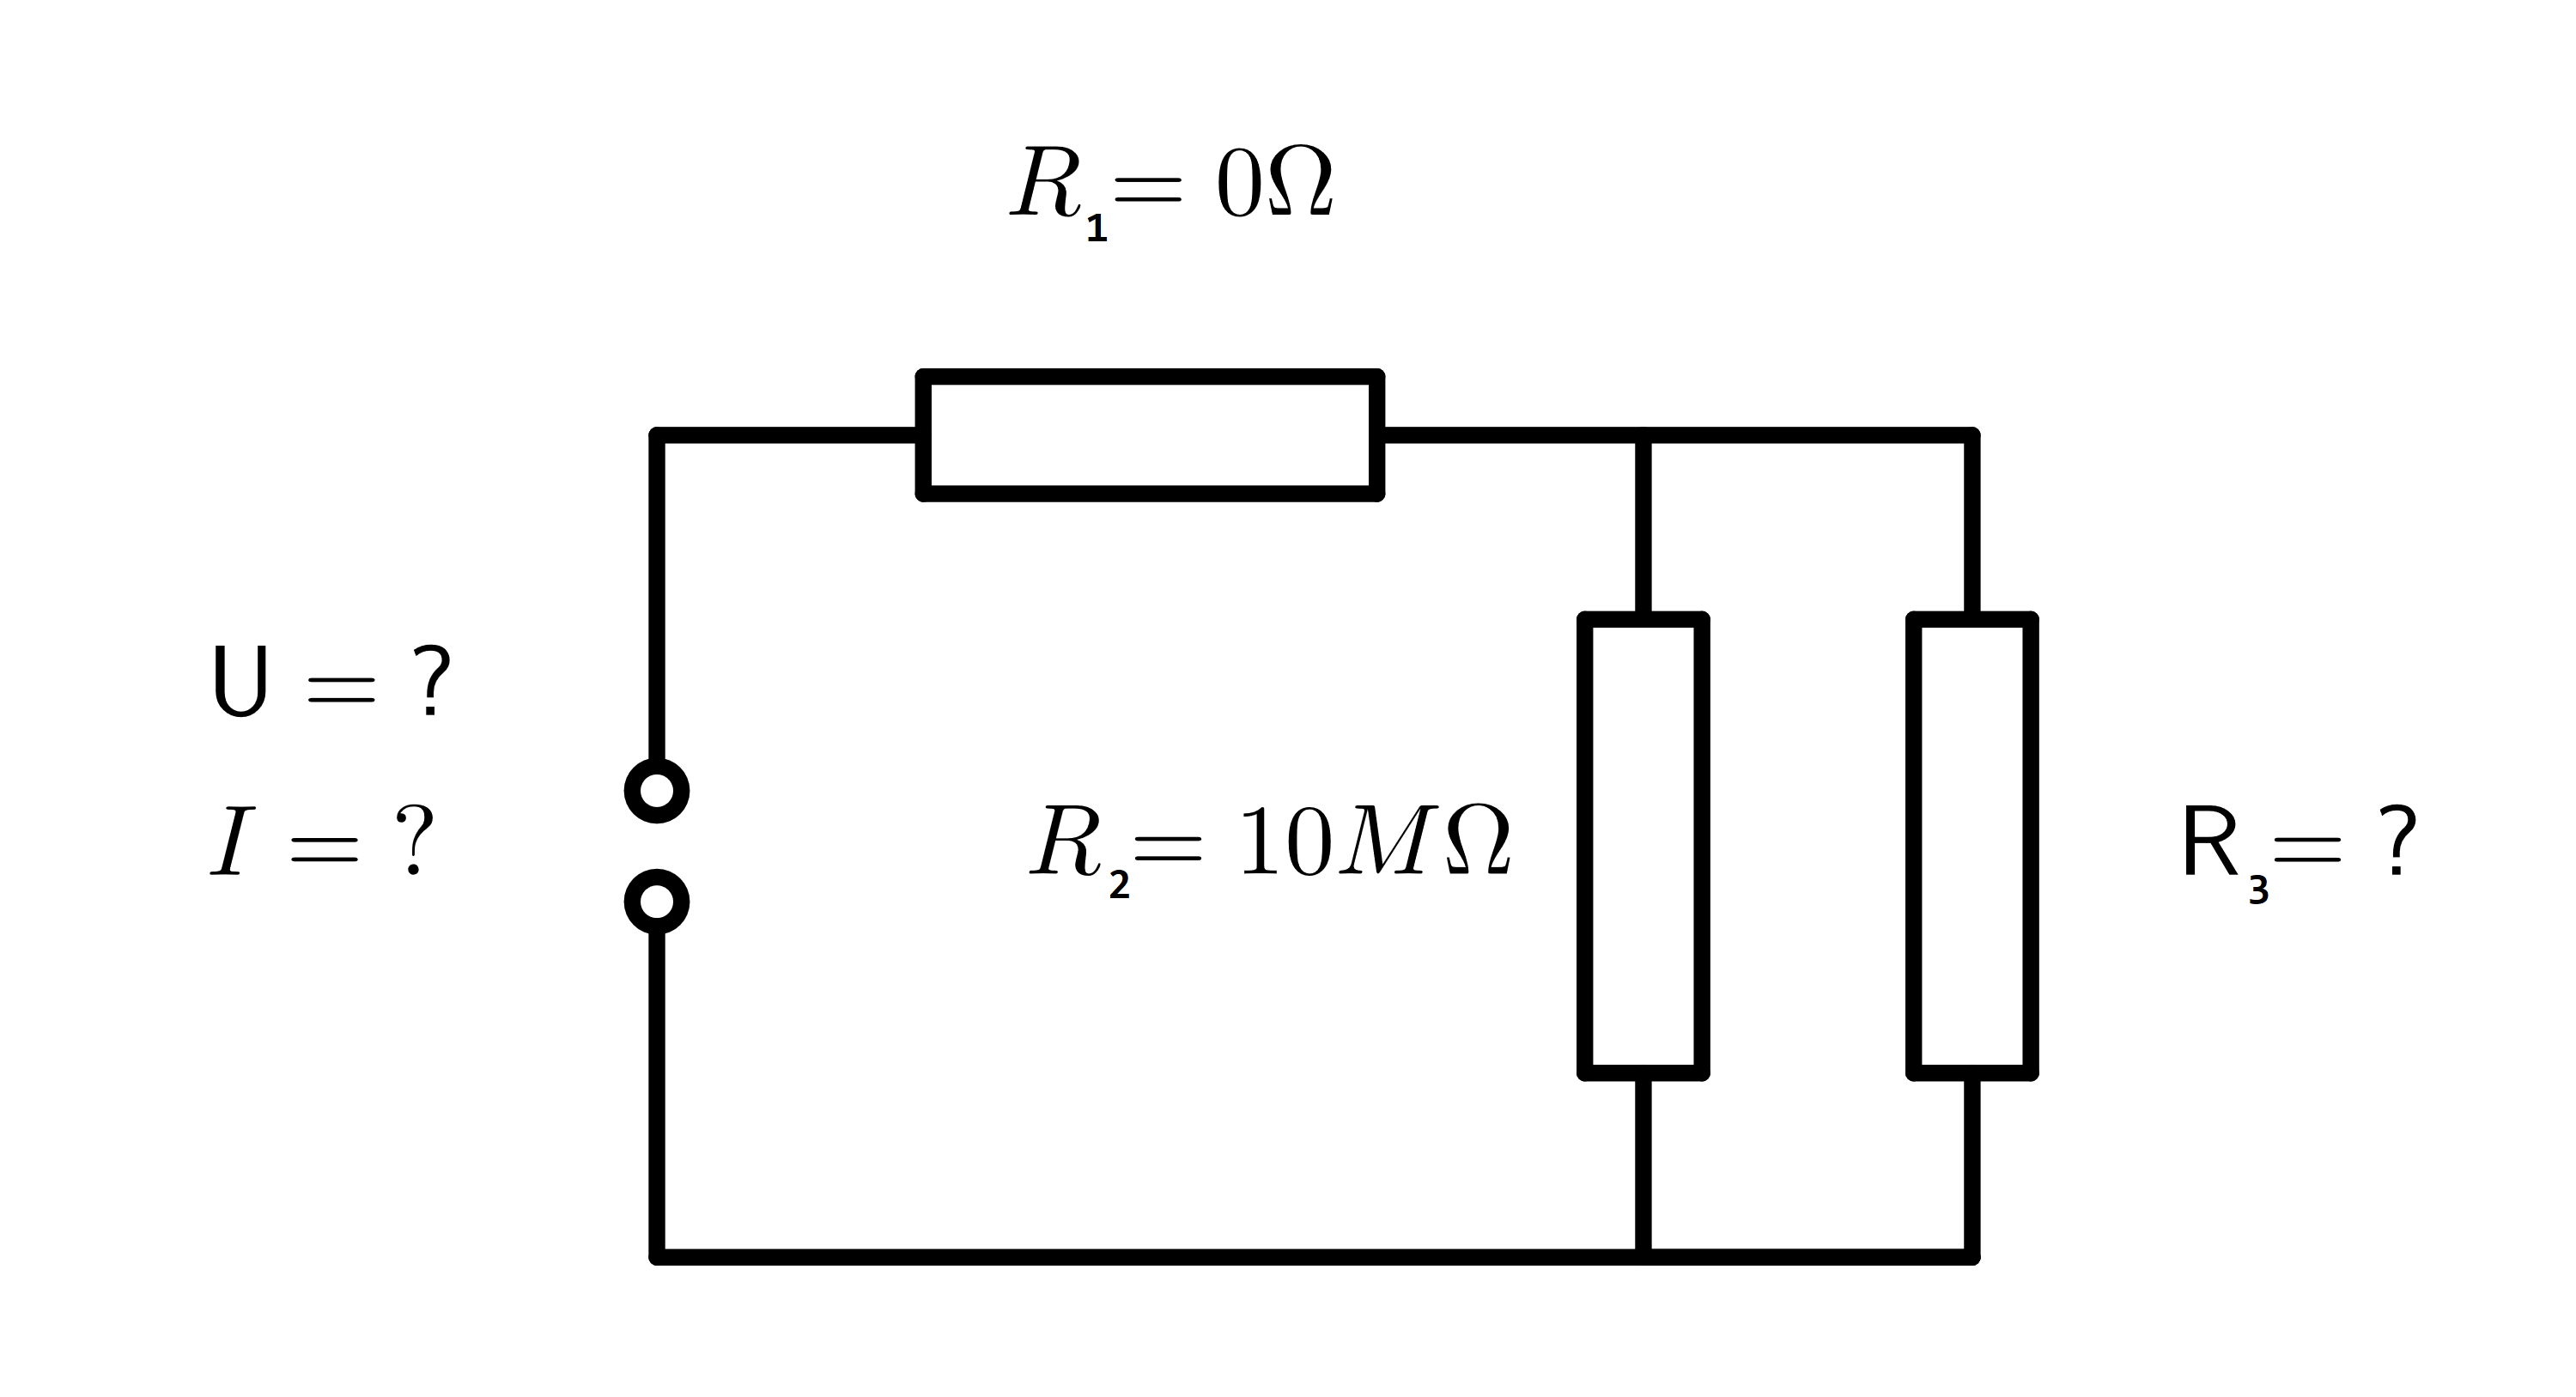
\includegraphics[width=\textwidth,height=0.2\textheight]{Bilder/ModellA.png}
\caption{Modell zur Schaltung a)}
\end{figure}

\textbf{\emph{Input:}}

Systemparameter:

\begin{itemize}
\tightlist
\item
  Spannung U an der Spannungsquelle
\item
  Stromstärke I im gesamten Stromkreis
\end{itemize}

Randbedingungen:

\begin{itemize}
\tightlist
\item
  Widerstand Amperemeter \(R_1\): \(0\Omega\)
\item
  Widerstand Voltmeter \(R_2\): \(10M\Omega\)
\end{itemize}

\textbf{\emph{Output:}}

\begin{itemize}
\tightlist
\item
  Widerstand des unbekannten Widerstandes \(R_3\)
\end{itemize}

\textbf{\emph{Modelldomäne}} Formel

\newpage

\textbf{\emph{Implementierung als R-Funktion mit zwei Argumenten:}}

\begin{Shaded}
\begin{Highlighting}[]
\CommentTok{\# {-}{-}{-}{-} Schaltung 1}
\CommentTok{\# INPUT: Spannung, Stromstärke}
\CommentTok{\# OUTPUT: Benötigter Widerstand}
\NormalTok{schaltung1 }\OtherTok{\textless{}{-}} \ControlFlowTok{function}\NormalTok{(U0, I0)\{}
  \CommentTok{\# Randbedingungen}
\NormalTok{  R1 }\OtherTok{=} \DecValTok{0} \CommentTok{\# Widerstand Amperemeter}
\NormalTok{  R2 }\OtherTok{=} \FloatTok{10e6} \CommentTok{\# Widerstand Voltmeter}
  \CommentTok{\# Berechnung des Gesamtwiderstandes}
\NormalTok{  Rges }\OtherTok{=}\NormalTok{ U0}\SpecialCharTok{/}\NormalTok{I0}
  \CommentTok{\# Berechnung des benötigten R}
\NormalTok{  R3 }\OtherTok{=}\NormalTok{ (}\DecValTok{1}\SpecialCharTok{/}\NormalTok{(Rges}\SpecialCharTok{{-}}\NormalTok{R1)}\SpecialCharTok{{-}}\DecValTok{1}\SpecialCharTok{/}\NormalTok{R2)}\SpecialCharTok{**{-}}\DecValTok{1}
  \FunctionTok{print}\NormalTok{(}\StringTok{"Widerstände in der Schaltung in Ohm:"}\NormalTok{)}
  \FunctionTok{print}\NormalTok{(}\FunctionTok{paste}\NormalTok{(}\StringTok{"R1: "}\NormalTok{, R1))}
  \FunctionTok{print}\NormalTok{(}\FunctionTok{paste}\NormalTok{(}\StringTok{"R2: "}\NormalTok{, R2))}
  \FunctionTok{print}\NormalTok{(}\FunctionTok{paste}\NormalTok{(}\StringTok{"R3: "}\NormalTok{, R3))}
  \FunctionTok{print}\NormalTok{(}\FunctionTok{paste}\NormalTok{(}\StringTok{"R\_ges: "}\NormalTok{, Rges))}
\NormalTok{\}}
\end{Highlighting}
\end{Shaded}

Wird das Modell mit den gemessenen Werten ausgeführt (das gemessene U
und I entsprechen bei Schaltung a) den Einstellungen an der
Spannungsquelle) erhält man mit diesem Modell folgenden Output:

\begin{Shaded}
\begin{Highlighting}[]
\CommentTok{\# Testen mit gemessenen Werten für Widerstand 1}
\FunctionTok{schaltung1}\NormalTok{(}\AttributeTok{U0=}\DecValTok{5}\NormalTok{, }\AttributeTok{I0=}\FloatTok{5.4e{-}06}\NormalTok{)}
\end{Highlighting}
\end{Shaded}

\begin{verbatim}
## [1] "Widerstände in der Schaltung in Ohm:"
## [1] "R1:  0"
## [1] "R2:  1e+07"
## [1] "R3:  1020408.16326531"
## [1] "R_ges:  925925.925925926"
\end{verbatim}

\begin{Shaded}
\begin{Highlighting}[]
\CommentTok{\# Testen mit gemessenen Werten für Widerstand 1}
\FunctionTok{schaltung1}\NormalTok{(}\AttributeTok{U0=}\FloatTok{0.15}\NormalTok{, }\AttributeTok{I0=}\FloatTok{0.1503}\NormalTok{)}
\end{Highlighting}
\end{Shaded}

\begin{verbatim}
## [1] "Widerstände in der Schaltung in Ohm:"
## [1] "R1:  0"
## [1] "R2:  1e+07"
## [1] "R3:  0.998004091617175"
## [1] "R_ges:  0.998003992015968"
\end{verbatim}

\end{document}
